	
	Se define la descomposición de \emph{Cholesky} como la matriz $X^{c}_k$ tal que:
	\begin{equation*}
		X_k = X^{c^{*}}_k X^{c}_k
	\end{equation*}	

	A partir de ello, se propone para el filtro de Kalman definir: 
	\begin{equation*}
		M_0 = \begin{bmatrix} R^{c}_k& C_k\; P^c_{k/k-1}& 0 \\[0.3em] 0& A_k\; P^c_{k/k-1}& B_k\; Q^c_k \end{bmatrix}
	\end{equation*}
	de modo que al factorizar $M^*_0 = Q\,R$ se obtiene que $A=R^* R$, es decir que $R$ es la factorización de \emph{Cholesky} de $A$. Para optimizar los cálculos, se le agrega una fila a dicha matriz para incorporar las mediciones. Entonces:
	\begin{equation*}
	M =  \begin{bmatrix} R^{c}_k& C_k\; P^c_{k/k-1}& 0 \\[0.3em] 0& A_k\; P^c_{k/k-1}& B_k\; Q^c_k \\[0.3em] -y^*\,R^{c^{-1}}_k & \hat{x}^*\, P^{c^{-1}}_{k/k-1} & 0 \end{bmatrix}
	\end{equation*}

	Como la matriz $R$ será triangular inferior (propiedad de la factorización \emph{QR}) se tiene:
	\begin{equation*}
	 \begin{cases} P_{k+1/k} = Z\,Z^*\\ \hat{x}_{k+1/k}=Z\,W^*_2\\ \hat{g}_k = -X\,W^*_1\end{cases} \text{ donde }\quad R^* = \begin{bmatrix} X&0&0\\[0.3em]Y&Z&0\\[0.3em]W_1&W_2&W_3\end{bmatrix}
	\end{equation*}

	Por lo tanto, el algoritmo de Kalman consta en calcular la matriz $M$ en cada iteración, realizar la factorización \emph{QR} y a partir de las submatrices de $R$ obtener las estimaciones de los estados, innovaciones y autocorrelación.

	Al correr el algoritmo se obtiene la trayectoria de la Figura \ref{fig:ej5}.

	\vspace*{\fill}

	\begin{figure}[H]
	\centering
	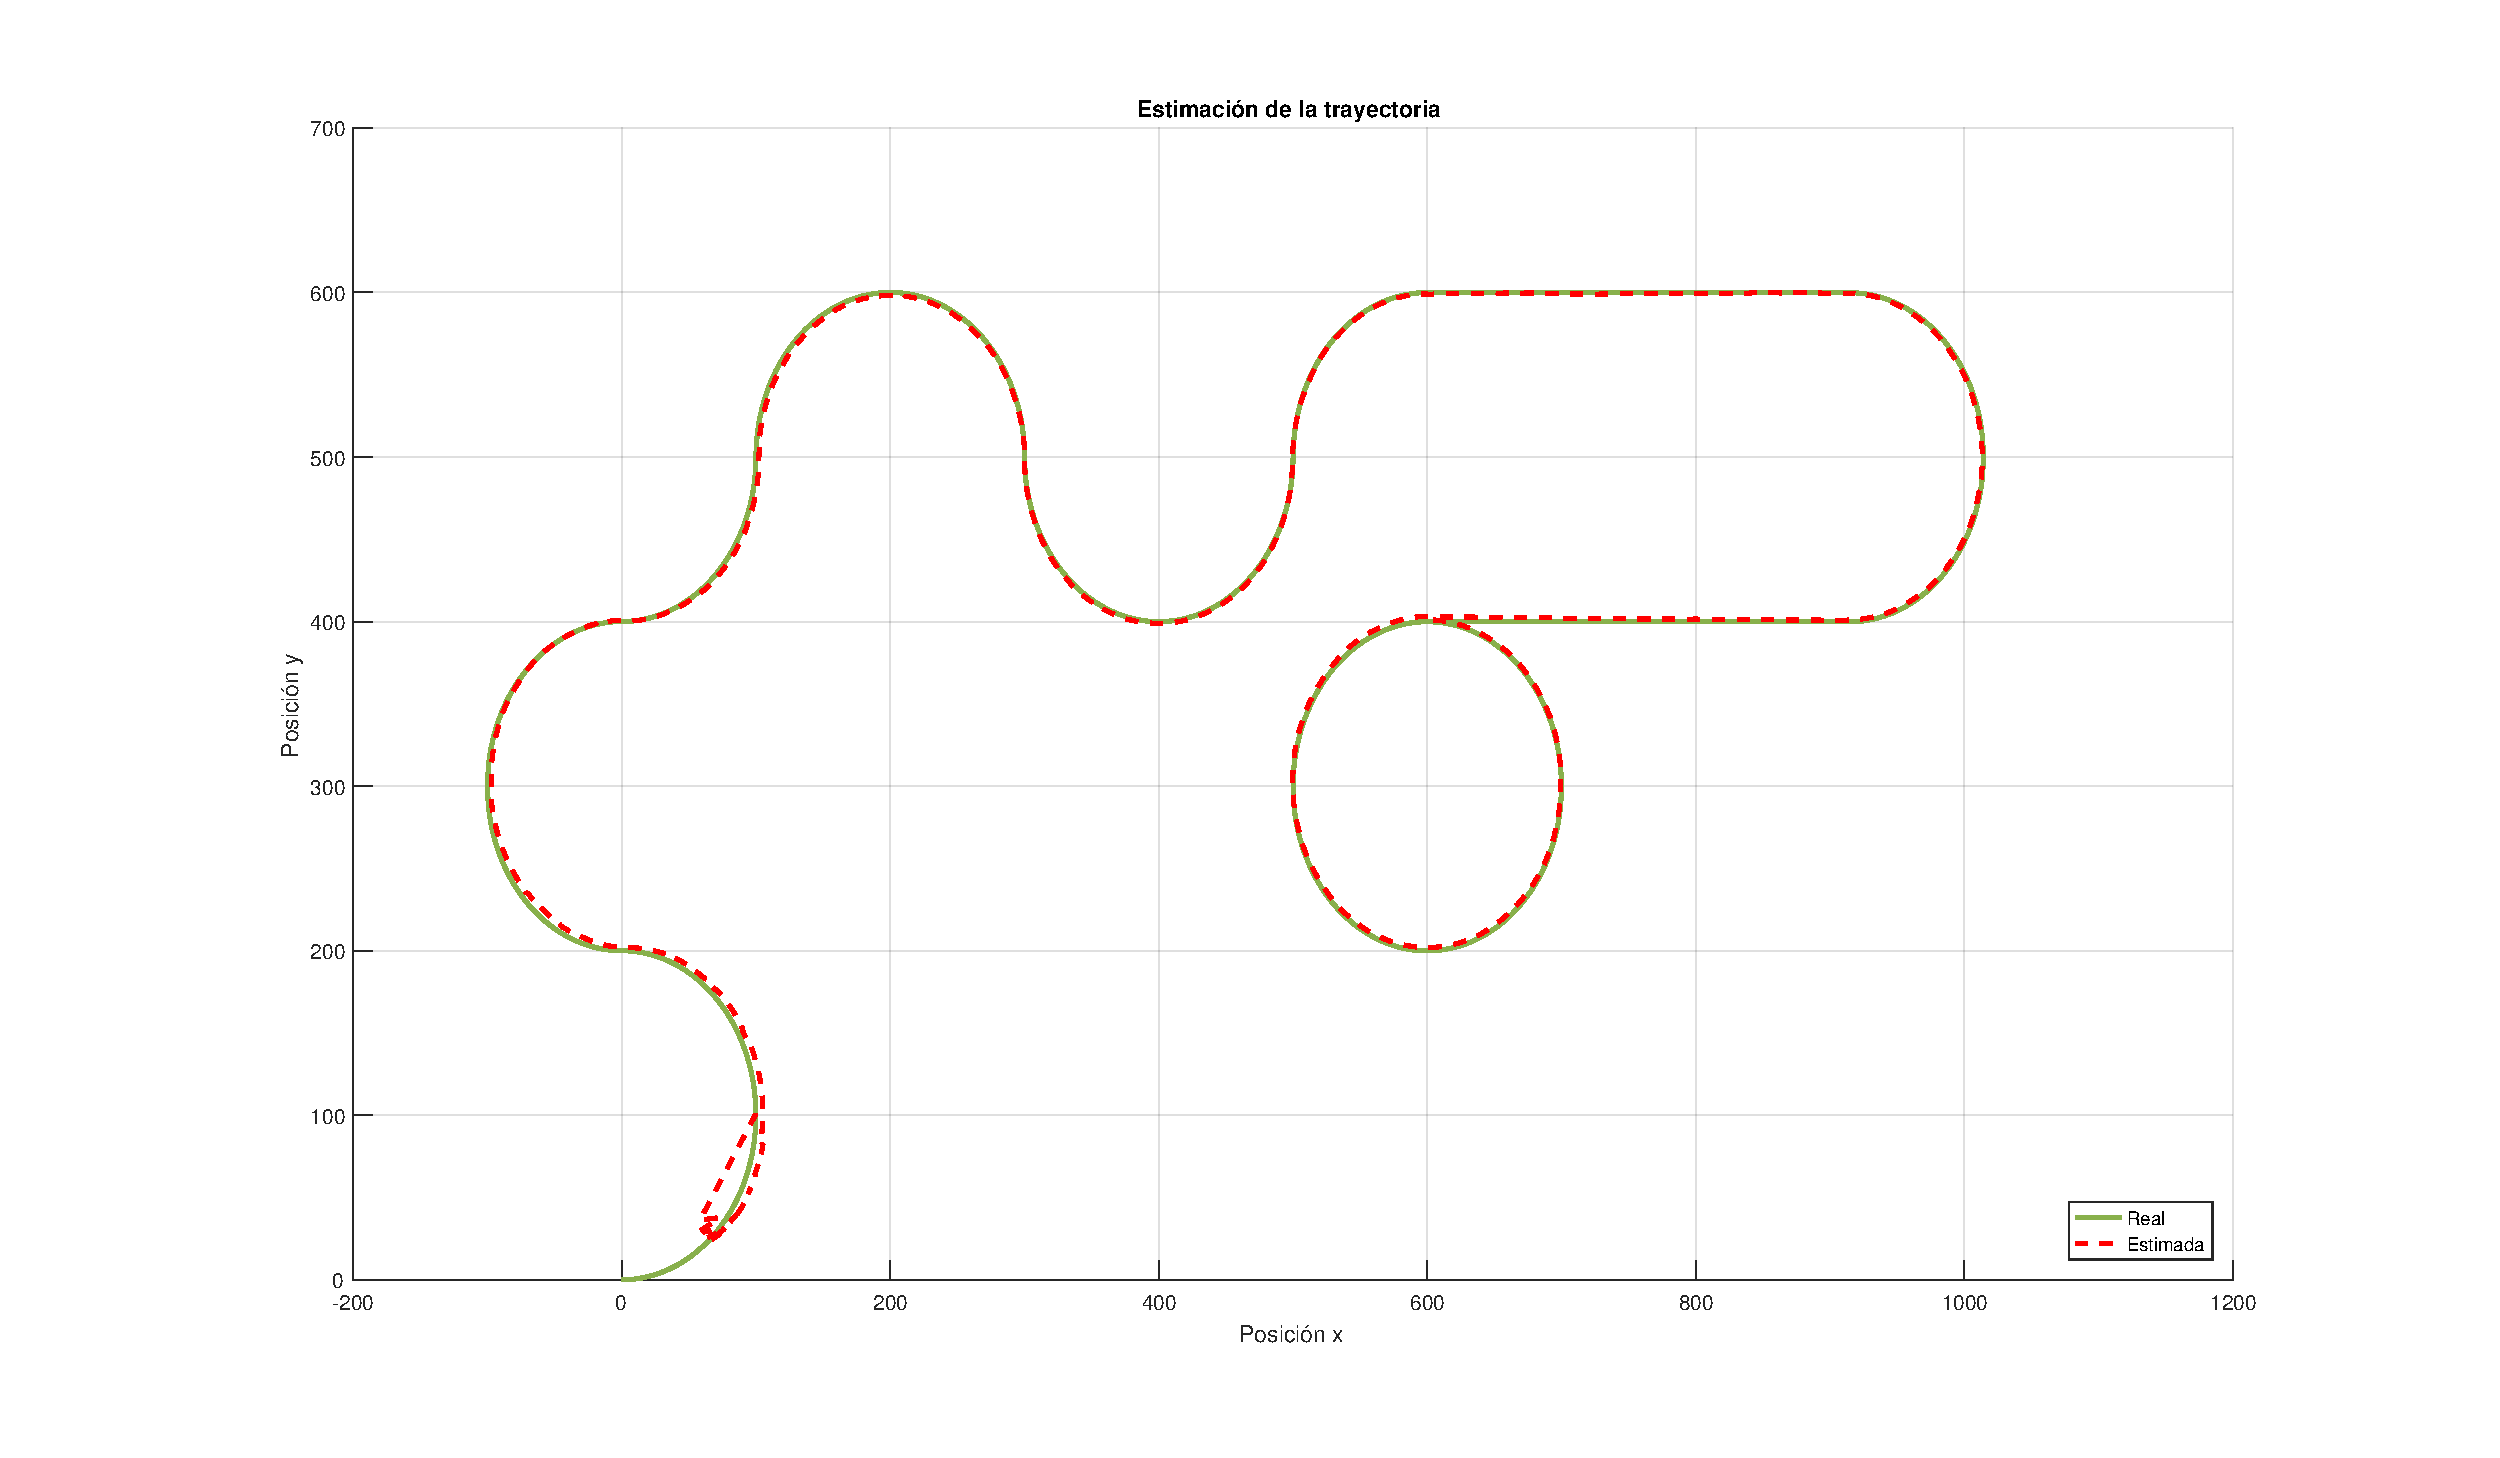
\includegraphics[width=\textwidth,trim= 1.5cm 1.5cm 1.5cm 1.5cm]{graf_ej5.pdf}
	\caption{Estimación de la trayectoria.}
	\label{fig:ej5} 
	\end{figure}

	\vspace*{\fill}
	\begin{figure}[H]
	\centering
	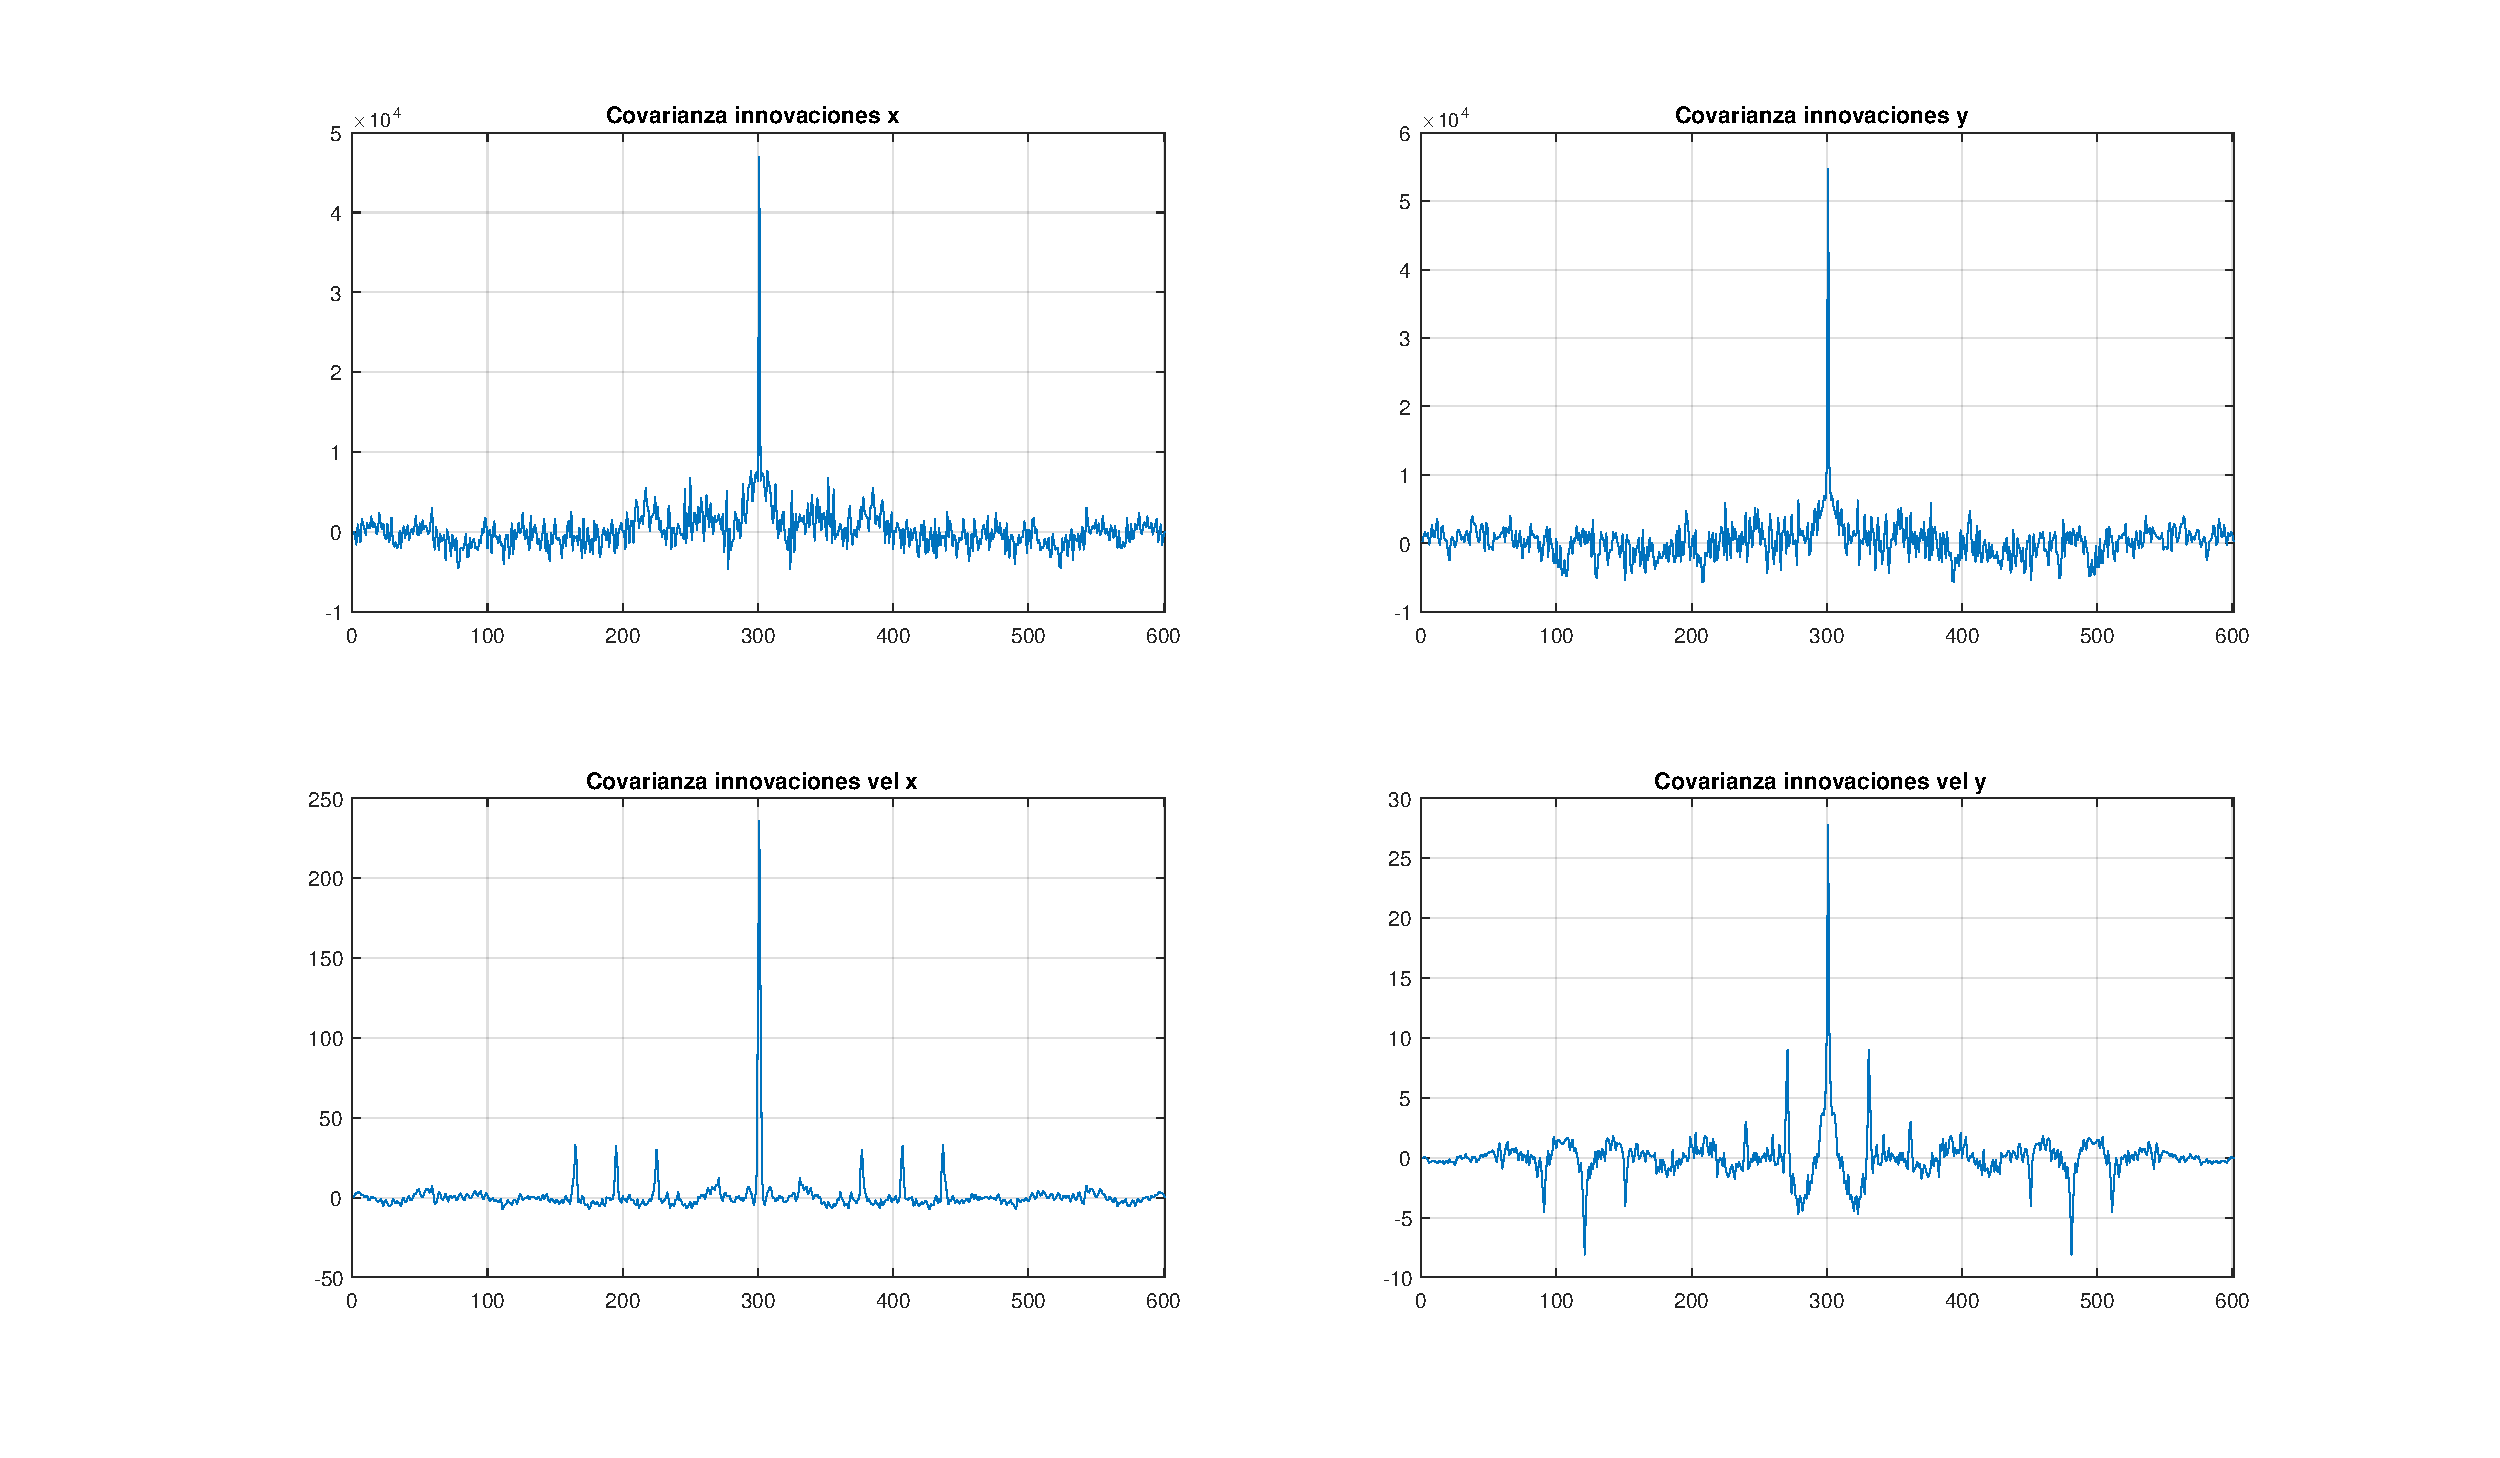
\includegraphics[width=\textwidth, trim=1.5cm 1.5cm 1.5cm 1.5cm]{graf_ej5_covinn.pdf}
	\caption{Covarianza de las innovaciones de las posiciones y velocidades en $x^e$ e $y^e$.}
	\label{fig:5covinn} 
	\end{figure}
	\vspace*{\fill}

	\pagebreak

	\vspace*{\fill}
	\begin{figure}[H]
	\centering
	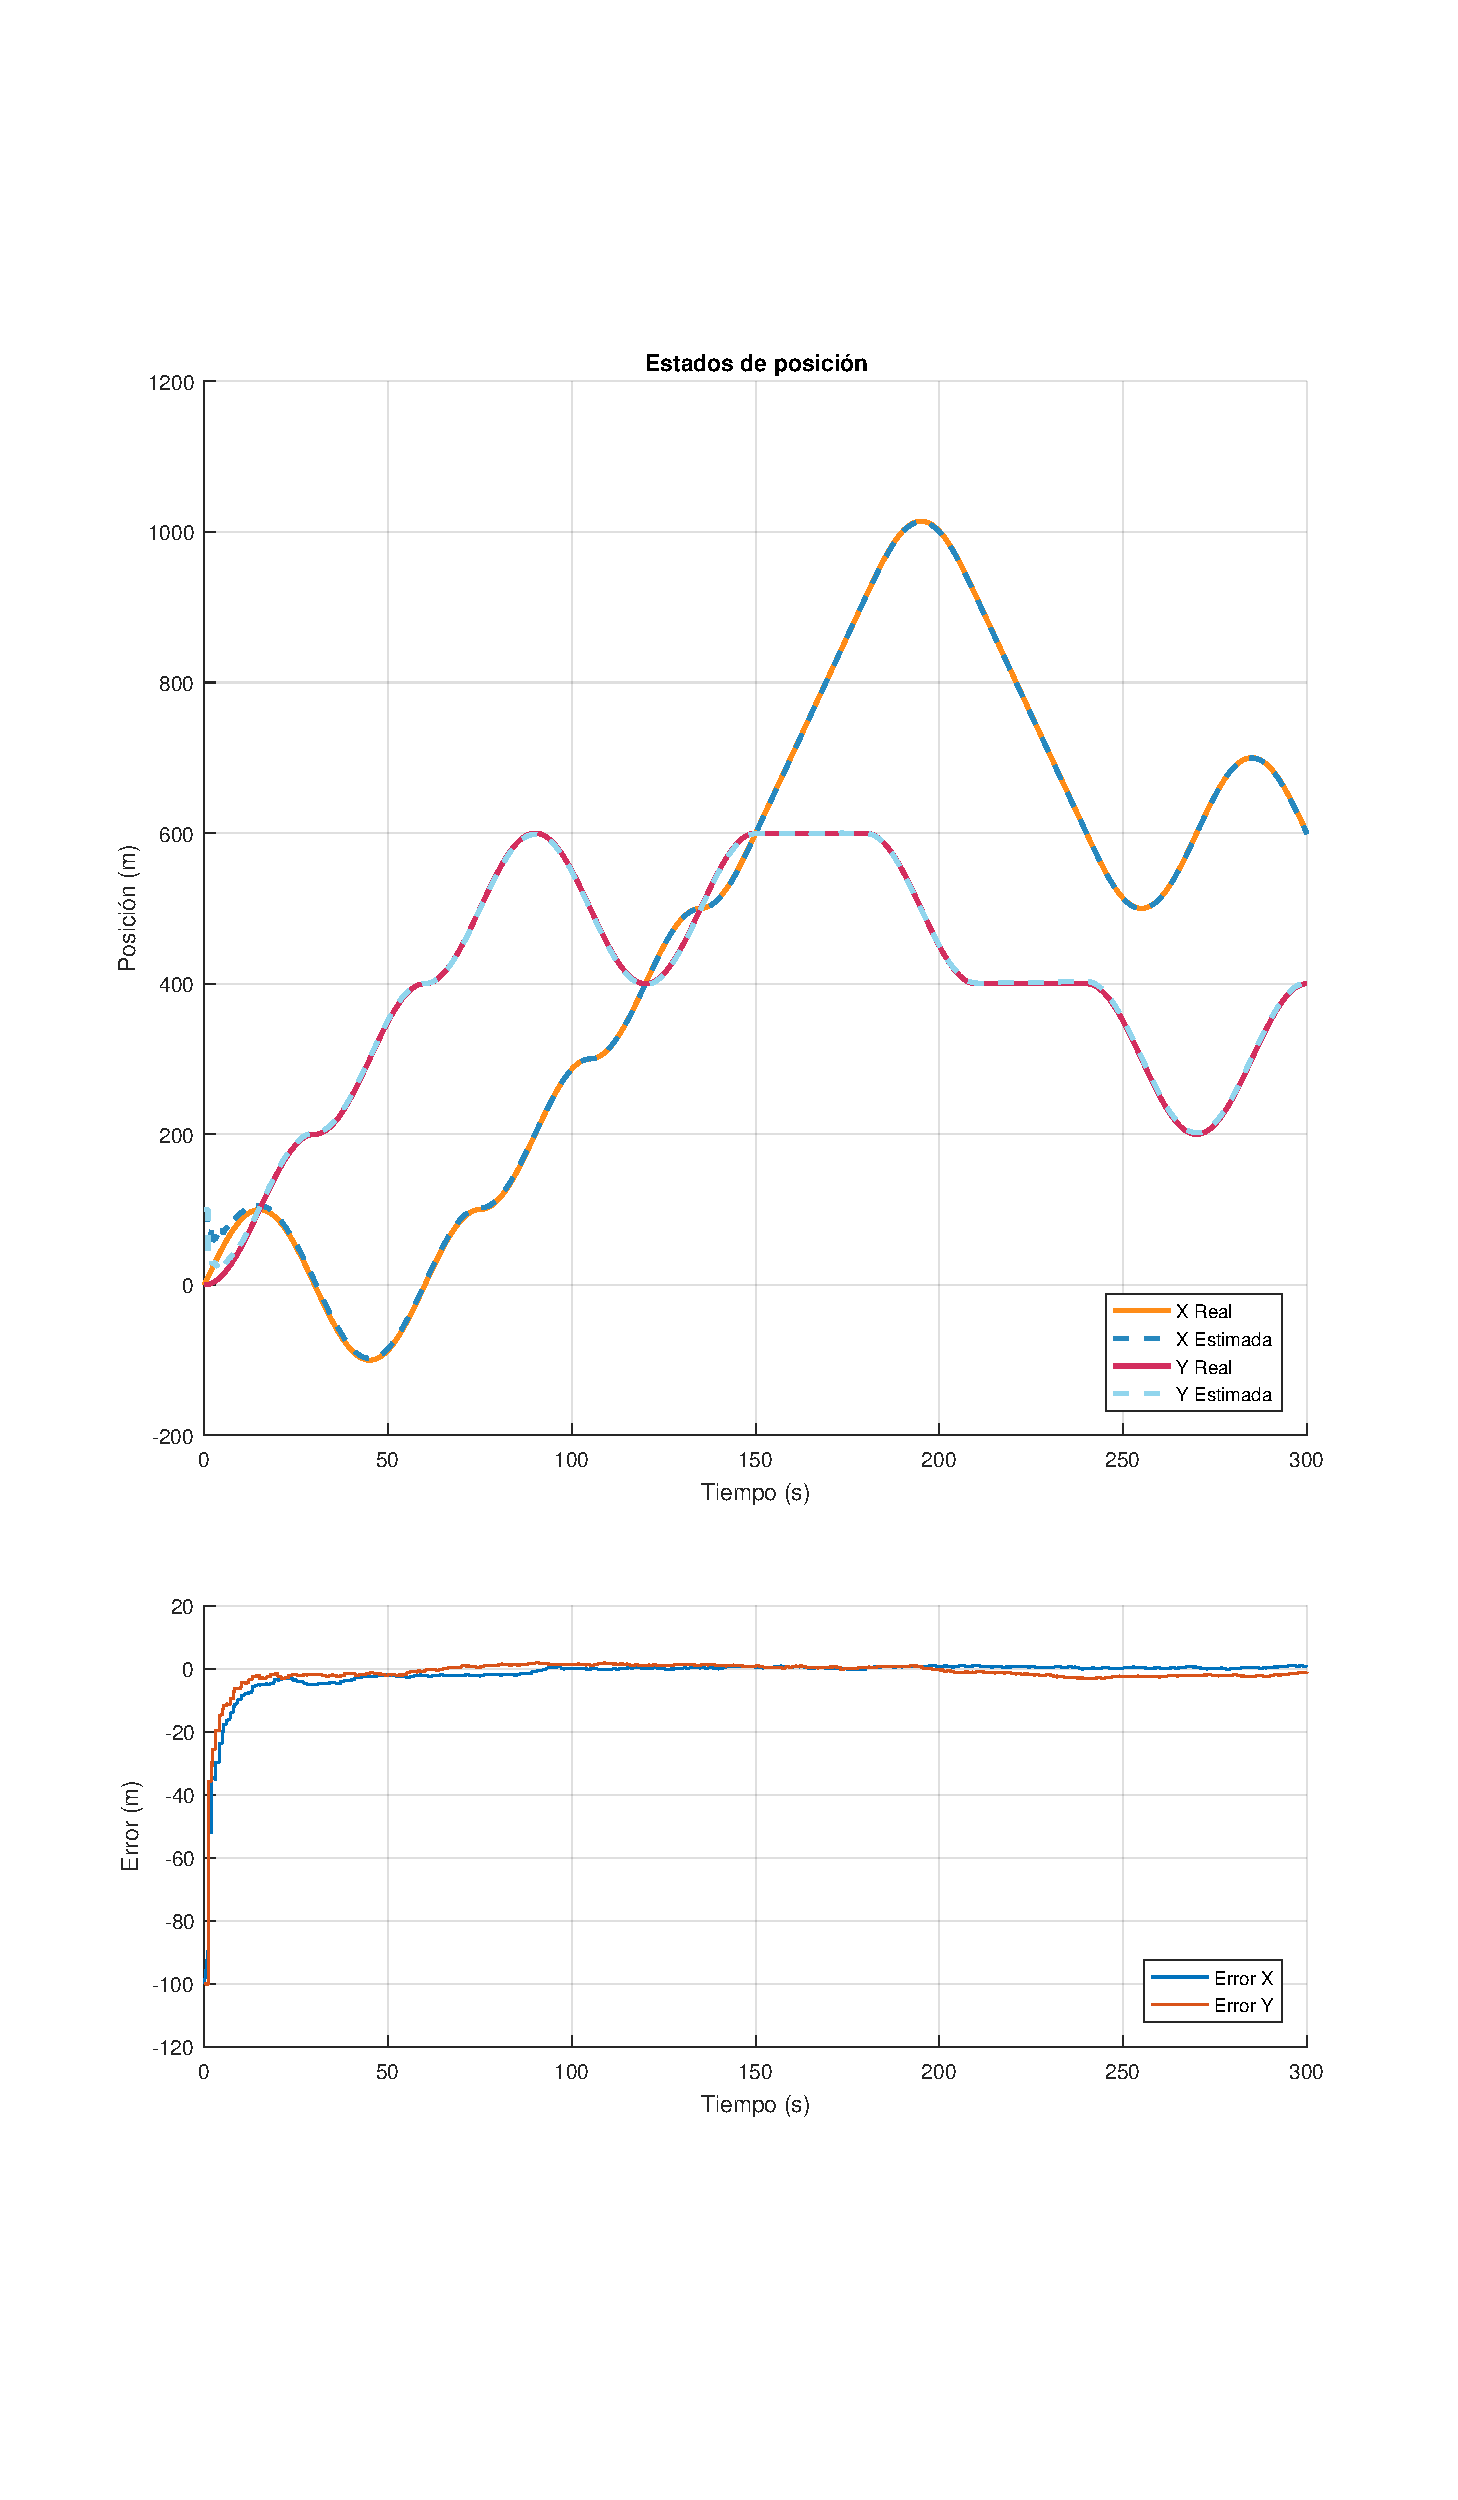
\includegraphics[scale=0.65, trim= 6cm 6cm 6cm 6cm]{graf_ej5_pos.pdf}
	\caption{Posición y error en función del tiempo.}
	\label{fig:5pos} 
	\end{figure}
	\vspace*{\fill}

	\pagebreak
	
	\begin{figure}[H]
	\centering
	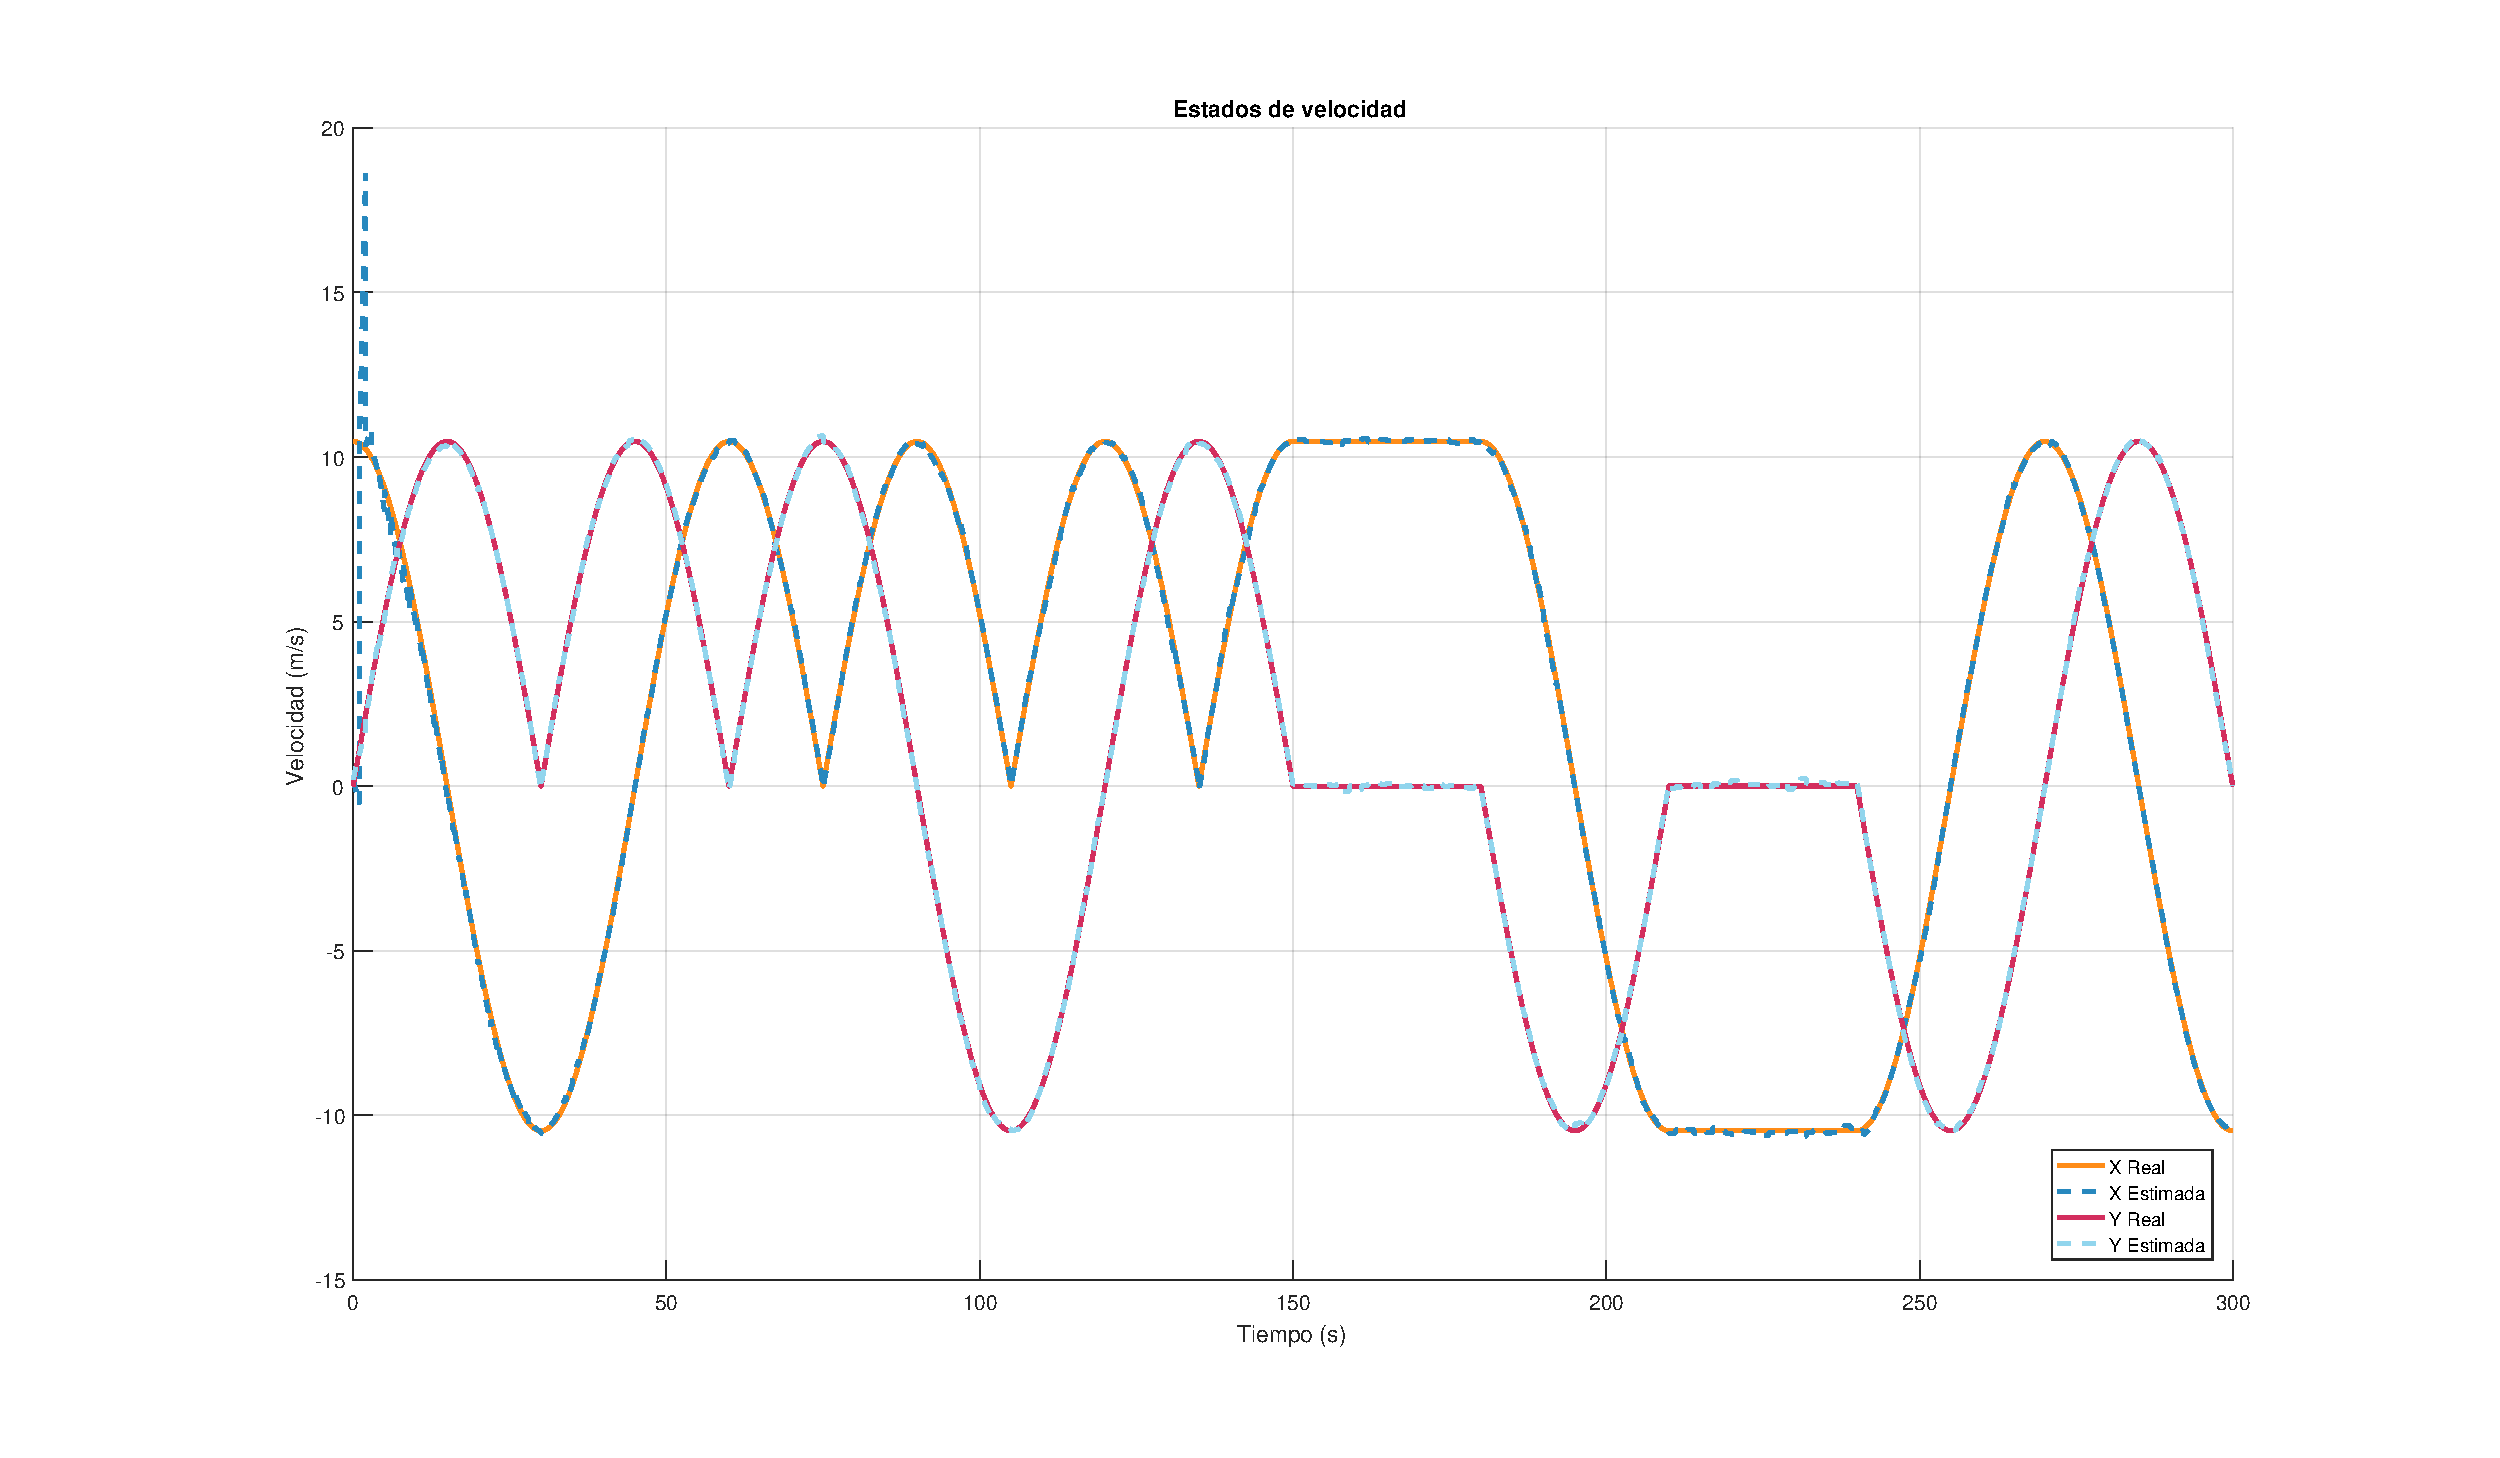
\includegraphics[width=0.9\textwidth, trim=1.5cm 1.5cm 1.5cm 1.5cm]{graf_ej5_vel.pdf}	
	\caption{Velocidad real y estimada en función del tiempo.}
	\label{fig:5vel} 
	\end{figure}

	\graficarPDF{graf_ej5_theta}{Valores de los coeficientes de $C^e_b$ en el tiempo.}{fig:5theta}

	

